%--------------------------------------------------------------------------
% Dokumentenklasse
%--------------------------------------------------------------------------

% disable Warning for remreset Package
% \RequirePackage{silence}
% \WarningFilter{remreset}{The remreset package}

\documentclass[
	pagesize,
	fontsize=12pt,
	paper=a4,
	oneside,
   reqno
]{scrartcl}

%--------------------------------------------------------------------------
% Standardpakete 
%--------------------------------------------------------------------------
\usepackage[ngerman]{babel}               % Deutsch Silbentrennung
\usepackage[T1]{fontenc}                  % Font Type
\usepackage[utf8]{inputenc}               % Font Encoding
\usepackage{lmodern}                      % Latin Modern Font
\usepackage{csquotes}                     % Setzen von Zitaten
\usepackage{xspace}                       % setzten von Leerzeichen nach Abkürzungen
\usepackage{microtype}                    % für glattere Seitenränder
\renewcommand*\familydefault{\sfdefault}  % Serifen lose Schrift
%\renewcommand*\familydefault{\ttdefault} % Schreibmaschinenschrift

%--------------------------------------------------------------------------
% Extra Packages
%--------------------------------------------------------------------------

% Abkürzungspaket
\usepackage{acronym}

% Symbolverzeichnis
\usepackage[symbols,nogroupskip,nonumberlist,sort=use]{glossaries-extra}

% \makenoidxglossaries

\glsxtrnewsymbol[description={Gewichtskraft}]{FG}{\ensuremath{F_{\mathrm{G}}}}
\glsxtrnewsymbol[description={Gewichtskraft in Bewegungsrichtung}]{FG1}{\ensuremath{F^{'}_{\mathrm{G}}}}
\glsxtrnewsymbol[description={Bewegungskraft des Schlittens}]{Fa}{\ensuremath{F_{\mathrm{a}}}}
\glsxtrnewsymbol[description={Pendelkraft}]{FP}{\ensuremath{F_{\mathrm{P}}}}
\glsxtrnewsymbol[description={Pendelkraft in Bewegungsrichtung}]{FP1}{\ensuremath{F^{'}_{\mathrm{P}}}}
\glsxtrnewsymbol[description={Reibkraft}]{Ff}{\ensuremath{F_{\mathrm{f}}}}
\glsxtrnewsymbol[description={Coulombsche Reibung}]{FC}{\ensuremath{F_{\mathrm{C}}}}
\glsxtrnewsymbol[description={Gesamtkraft}]{Fges}{\ensuremath{F_{\mathrm{ges}}}}
\glsxtrnewsymbol[description={Pendelmoment}]{MP}{\ensuremath{M_{\mathrm{P}}}}
\glsxtrnewsymbol[description={Gewichtsmoment}]{MG}{\ensuremath{M_{\mathrm{G}}}}
\glsxtrnewsymbol[description={Reibmoment}]{Mf}{\ensuremath{M_{\mathrm{f}}}}
\glsxtrnewsymbol[description={Gesamtmoment}]{Mges}{\ensuremath{M_{\mathrm{ges}}}}

% Mathe Pakete
\usepackage{amsmath}
\DeclareMathOperator{\sgn}{sgn}
\usepackage{thmtools}
\usepackage{amsfonts}
\usepackage{amssymb}
\usepackage{mathtools}
\usepackage{breqn}

% Listenumgebungen
\usepackage{listings}
\usepackage{paralist}
\usepackage{enumitem}
\usepackage{adjustbox}

% Demo Text
\usepackage{blindtext}

% Farb-Pakete
\usepackage{xcolor}
\usepackage{fancyvrb}
\usepackage{colortbl}

% Farbedefinitionen
\definecolor{htw}{RGB}{120, 184, 2}
\definecolor{ccW}{RGB}{255,255,255}
\definecolor{ccR}{RGB}{197,14,31}
\definecolor{ccG}{RGB}{113,113,113}
\definecolor{ccL}{RGB}{220,220,220}
\definecolor{ccS}{RGB}{0,0,0}
\definecolor{ccB}{RGB}{68,73,159}
\definecolor{ccD}{RGB}{0,0,80}

% Für erweiterte Tabellen
\usepackage{longtable}
\usepackage{tabularx}
\usepackage{float}
\usepackage{multirow}
\usepackage{makecell}
% \setlength{\tabcolsep}{0.5em}       % for the horizontal padding
% {\renewcommand{\arraystretch}{1.8}  % for the vertical padding
% \usepackage{ragged2e}
% \newcolumntype{R}[1]{>{\RaggedRight}p{#1}}

% Einheitenpaket
\usepackage[exponent-product = \cdot]{siunitx}
\sisetup{locale=DE}

\makeatletter
\renewcommand\@dotsep{5}
\makeatother

% Pakete für Grafiken
\usepackage{graphicx}
\usepackage{wrapfig}
\usepackage{overpic}
\usepackage{epstopdf}
\usepackage{caption}
\usepackage{subcaption}
\usepackage{rotating}
\usepackage{lscape}
% \captionsetup[subfigure]{list=true, font=normalsize, labelformat=brace, position=top} %setup für subfigure captions

% Diagramm-/Grafikerstellung
\usepackage{pstricks}
\usepackage{tikz}
\usetikzlibrary{math}
\usepackage{pgfplots}
\pgfplotsset{compat=1.5}
\usetikzlibrary{intersections,positioning,arrows,automata,calc,patterns,shapes.multipart,fit,backgrounds,decorations.pathreplacing}
\usetikzlibrary{decorations,shapes.geometric}
\usetikzlibrary{matrix,calc,angles,positioning,quotes}
% \usepackage{tikz-uml}

\usepackage{pgfkeys}
\usepackage{pgfopts}
\usepackage{ifthen}
\usepackage{xstring}
\usepackage{calc}
\usepackage{pst-plot,pst-bar,pst-node} % Balkendiagramme
\usepackage{capt-of}
\usepackage{incgraph} % Fullscreen Images
\usepackage{pdfpages} % Include external pdf pages

\usepackage{latexsym}
\usepackage{censor}
\usepackage{here}
% \StopCensoring        % Auskommentiert wird der Text entschwaerzt 
% \censor{Oszilloskop}  % Befehl zum einschwärzen
\usepackage{trfsigns}   % Transformation Symbol o---o \laplace and \Laplace
\usepackage{circuitikz}

\usepackage{multido}

% Verlinkungen im Text
\usepackage{url}
\usepackage{hyperref}
\PassOptionsToPackage{hyphens}{url}
\hypersetup{hidelinks}
\urlstyle{same}

%--------------------------------------------------------------------------
% Eigene Befehle
%--------------------------------------------------------------------------
% Test 
% \renewcommand{\thesection}{\arabic{section}} % Section startet mit 1.0 und nicht mit 0.1

%------------sectioning command-------------------
% The sectioning command one level down the hierarchy from \subsubsection is called \paragraph followed by \subparagraph
% to include this in your table of contents

% for paragraph
\setcounter{tocdepth}{4}
\setcounter{secnumdepth}{4}
% for subparagraph
\setcounter{tocdepth}{5}
\setcounter{secnumdepth}{5}

% Abkürzungen durch Kommandos setzen
\newcommand{\bspw}{bspw.\xspace}
\newcommand{\bzw}{bzw.\xspace}
\newcommand{\etc}{etc.\xspace}
\newcommand{\zB}{z.\,B.\xspace}
\newcommand{\EV}{e.\,V.\xspace}
\newcommand{\zT}{z.\,T.\xspace}
\newcommand{\iVm}{i.\,V.\,m.\xspace}
\newcommand{\idR}{i.\,d.\,R.\xspace}
\newcommand{\ihv}{i.\,H.\,v.\xspace}
\newcommand{\ua}{u.\,a.\xspace}
\newcommand{\dH}{d.\,h.\xspace}
\newcommand{\vgl}{vgl.\xspace}
\newcommand{\ca}{ca.\xspace}
\newcommand{\dV}{d.\,Verf.}
\newcommand{\RNr}{Rn.\xspace}
\newcommand{\oa}{o.\,{ä}.\xspace}
\newcommand{\vC}{v.\,Chr.\xspace}
\newcommand{\nC}{n.\,Chr.\xspace}
\newcommand{\vA}{v.\,a.\xspace}
\newcommand{\eng}{engl.\xspace}
\newcommand{\tabitem}{~~\llap{\textbullet}~~}

%------------Zitate-------------------------------
\newcommand*{\zitat}[2]{%
   \normalfont\small
   \begin{quote}
   \glqq#1\grqq \par
   #2
   \end{quote}
   \normalsize
}
\newcommand*{\zitatmitueberschrift}[3]{%
   \normalfont\small
   \begin{quote} #3
   \glqq#1\grqq \par
   #2
   \end{quote}
   \normalsize
}
\newcommand*{\zitext}[2]{%
   \glqq#1\grqq\ %
   [#2]%
}

%-----------Seitendesign--------------------------
\usepackage[width=15.5cm, height=23cm, includeheadfoot]{geometry}
\geometry{paper=a4paper}
% \usepackage[left=6cm,right=1cm,top=1.5cm, bottom=1cm, includeheadfoot]{geometry}
% \newgeometry{oneside}
% \setlength{\voffset}{0cm}
\setlength{\headheight}{1.1\baselineskip} % increase headheight
\setlength{\footheight}{28.99998pt}       % increase foodheight
\setlength{\parindent}{0cm}               % Einrücken nach \newline
\setlength{\footskip}{86pt}               % Move Footer down
% \setlength{\topmargin}{0cm}
% \setlength{\marginparsep}{0.5cm}
% \setlength{\marginparwidth}{1.5cm}
% \setlength{\textwidth}{16cm}
% \setlength{\textheight}{23cm}
% \setlength{\oddsidemargin}{1cm}
% \setlength{\evensidemargin}{2cm}

%----------Kopf & Fußzeile------------------------
% \usepackage[headsepline,footsepline]{scrpage2}
\usepackage[headsepline]{scrlayer-scrpage}
\pagestyle{scrheadings}
\clearpairofpagestyles
\ihead{\headmark}
\automark{section}
\chead{}
\ohead{
\includegraphics[scale=0.09]{Bilder/HTWLogoKopfzeile.png} \nocite{HTWklein}}
\ifoot{Sebastian Richter\\ Aaron Zielstorff}
\cfoot{\pagemark}
\ofoot{VA2 Hochverfügbare\\ und sichere Systeme}

%--------------------------------------------------------------------------
% Beginn des Dokuments
%--------------------------------------------------------------------------
\begin{document}

%----------Deckblatt----------------------------- 
\begin{titlepage}
   \pagestyle{empty} % setzt Pagestyle-Befehl

   % HTW Logo
   \begin{flushright}
   
\includegraphics[scale=.07]{Bilder/LogoHTWBerlin.png}  \nocite{HTWgross}
   \end{flushright}

   \vspace{1cm}

   % Titel
   \begin{center}
      \Huge{\textbf{Konzeption und Realisierung eines Laborversuches im Modul:
VA2 Hochverfügbare und sichere Systeme}} \\
   \end{center}

   \vspace{3cm}

   % Name
   \begin{flushleft}
      \begin{tabular}{l c l }
         \textbf{Name: }&\hspace{1 cm} &\textbf{Matrikelnummer:} \\
         Sebastian Richter  & & 572906 \\
         Aaron Zielstorff   & & 567183 \\
      \end{tabular}
   \end{flushleft}

   \vspace{1cm}

   % Daten
   \begin{tabular}{l l}
      \textbf{Fachbereich:}   & FB1                                                 \\
      \textbf{Studiengang:}   & M.\xspace Elektrotechnik                            \\
      \textbf{Fachsemester:}  & 2.\xspace FS                                        \\
      \textbf{Fach:}          & VA2 Hochverfügbare und sichere Systeme              \\
      \textbf{Dozent:}        & Prof.\xspace Dr.\xspace -Ing.\xspace Stephan Schäfer\\
      \textbf{Abgabe am:}     & 23.\xspace September 2022                           \\ 
   \end{tabular}
\end{titlepage}
\clearpage

%--------Inhaltsverzeichnis-----------------------
\renewcommand{\contentsname}{Inhaltsverzeichnis}
\tableofcontents
\clearpage

%--------Abbildungsverzeichnis--------------------
% \renewcommand{\listfigurename}{Abbildungsverzeichnis}
% \renewcommand*{\figurename}{Abb.}
% \listoffigures
% \clearpage

%--------Tabellenverzeichnis----------------------
% \renewcommand*{\listtablename}{Tabellenverzeichnis}
% \renewcommand*{\tablename}{Tab.}
% \listoftables
% \clearpage

%----------Symbolverzeichnis----------------------
% \printnoidxglossary[type=symbols,style=long,title={Symbolverzeichnis}]
% \clearpage

%---------Kapitel/Text----------------------------

\section{Einführung}

Es sollen Fähigkeiten und Fertigkeiten für den Programmentwurf für sicherheitsgerichtete Anlagenmodelle (Funktionale Sicherheit nach DIN EN 61131-6) unter Verwendung von Beschreibungsmitteln und der Programmierung (Normsprachen nach DIN EN 61131-3) am Beispiel eines Silos mit Fördereinrichtung aufgebaut werden. Hierzu sollen zunächst unter Verwendung der textbasierten Programmiersprache \glqq Strukturierter Text, ST\grqq{} sicherheitsgerichtete Programmelemente entwickelt werden. Für diesen Zweck wird die Siemens S7-1500 Industriesteuerung inklusive der dezentralen Peripherie ET 200 SP und deren Programmierumgebung TIA Portal V17 verwendet.

\section{Voraussetzungen}

Um die nachfolgend beschriebene Anlage in Betrieb nehmen und Fehler simulieren zu können, wird ein Bachelor-Abschluss in Elektrotechnik oder in einem anderen ingenieurwissenschaftlichen Studiengang vorausgesetzt. Zusätzlich wird das Wissen aus den Vorlesungen der Bachelor-Module \glqq Grundlagen der Automation\grqq{}, \glqq Prozesssteuerungssysteme\grqq{} und \glqq Projekt: Prozesssteuerungssysteme\grqq{} und der Nachweis der erfolgreichen Teilnahme an den jeweiligen Laborpraktika verlangt. Durch die erfolgreiche Teilnahme weist der Studierende die notwendigen Fähigkeiten im Bereich der ST-Programmierung nach.

\section{Anlagenbeschreibung}

\begin{figure}[H]
   \centering
   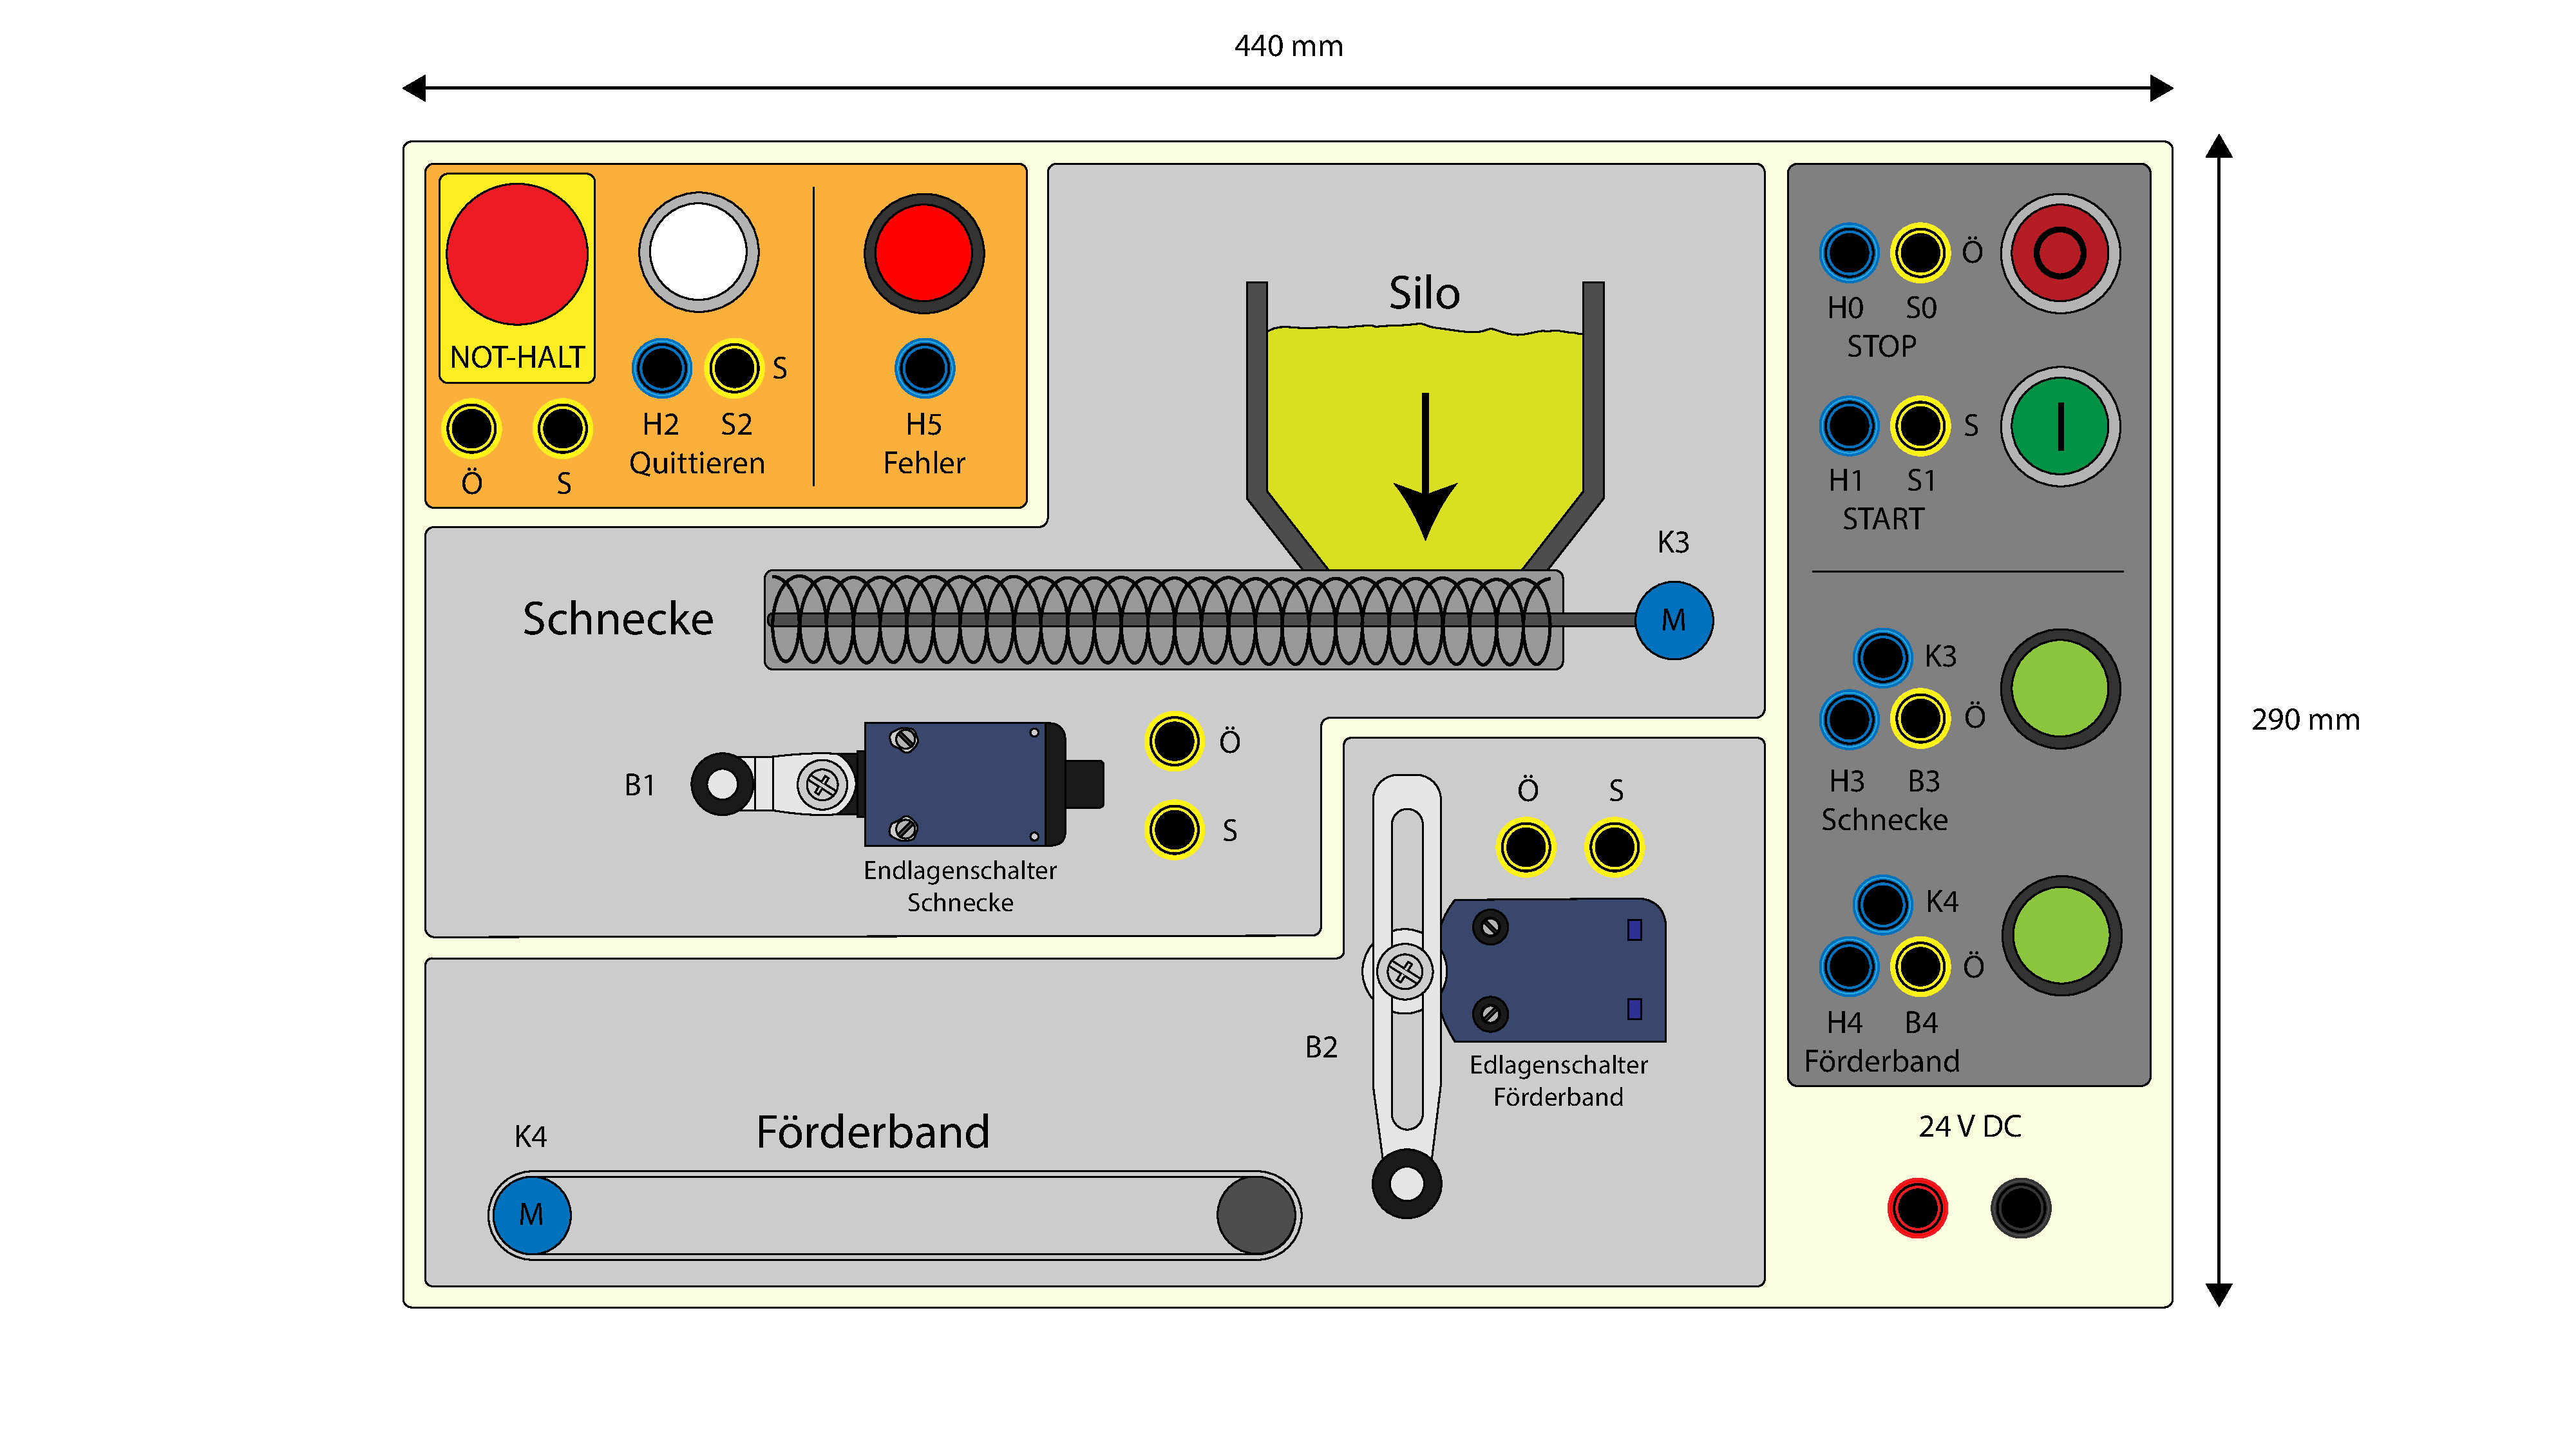
\includegraphics[width=1.0\textwidth]{Bilder/Aufbauplan_Vorderseite.pdf}
   \caption[Technologieschema]{Technologisches Schema der Anlage \glqq Silo mit Förderanlage\grqq{}}
   \label{fig:Bild1}
\end{figure}

Die Versuchsanlage kann sich grundsätzlich in drei Betriebszustände befinden. Dabei handelt es sich um den \textbf{betriebsbereiten Zustand}, den \textbf{Normalbetrieb} und den \textbf{Fehlerfall}. Diese sind nachfolgend beschrieben.

\subsection{Betriebsbereiter Zustand}

Zunächst muss die Stromversorgung hergestellt werden. Der betriebsbereite Zustand wird erreicht, wenn für die Anlage kein Fehler detektiert wird. Zusätzlich dürfen die Endlagen der Förderschnecke und des Förderbandes (B1, B2) nicht auslösen. Die Motoren müssen ausgeschaltet sein, d.h. die SPS erhält FALSE-Signal der Hilfskontakte (B3, B4) der Schütze.\\
Sind die vorangegangenen Bedingungen erfüllt, blinkt der START-Leuchtdrucktaster (H1) mit einer vorgegeben Frequenz von f = 1 Hz. Der STOP-Leuchtdrucktaster (H0) ist ausgeschaltet.

\subsection{Normalbetrieb}

Die Anlage wird durch das Drücken des START-Leuchtdrucktasters (S1) vom betriebsbereiten Zustand in den Normalbetrieb überführt. Der START-Leuchtdrucktaster (H1) hört zu blinken auf und leuchtet nun dauerhaft. Der STOP-Leuchtdrucktaster (H0) leuchtet ebenfalls dauerhaft. Befindet sich die Anlage im Normalbetrieb, soll der Prozess des Materialtransportes von einer Förderschnecke über ein Förderband simuliert werden. Die Ansteuerung der Förderschnecke und des Förderbandes erfolgt jeweils über eine zugeordnete Motorsteuerung. Die modellhaft dargestellten Motoren werden über Hilfsschütze (K3, K4) angesteuert. Der Schaltzustand der Schütze (B3, B4) wird über Hilfskontakte einerseits zur weiteren Auswertung auf die SPS (S7-1500) rückgeführt, andererseits erfolgt die Signalisierung an den Anwender mittels Leuchtmelder (H3, H4). Damit ein fehlerfreier Transport gewährleistet wird, muss das Förderband vier Sekunden vor der Schnecke anlaufen. Ebenfalls ist ein Nachlauf des Förderbandes von fünf Sekunden nach dem Stoppen der Förderschnecke erforderlich. \\
Die Anlage besitzt sowohl für die Förderschnecke als auch das Förderband einen mechanischen Endlagensensor (B1, B2). Das Erreichen der Endlagen wird der SPS signalisiert. \\
Die Anlage wird durch das Drücken des STOP-Leuchtdrucktasters (S0) angehalten.

\subsection{Fehlerfall}

Tritt ein vom Normalbetrieb abweichender Anlagenzustand auf, wird dieser über die Steuerung bzw. das Steuerungsprogramm erkannt und über das Blinken des FEHLER-Leuchtmelders (H5) signalisiert (Blinktakt 1 Hz). Weiterhin findet ein NOT-Halt statt, so dass keine Gefährdung mehr von der Anlage ausgeht. Der Nutzer muss anschließend den Fehler beheben und diesen über einen QUITTIER-Taster (S2) bestätigen. Aus Sicherheitsgründen sollen sowohl kritische als auch unkritische Fehler quittiert werden. Die Anlage befindet sich nun wieder im betriebsbereiten Zustand. Über das erneute Betätigen des START-Leuchtdrucktasters (S1) nimmt die Anlage ihren Normalbetrieb wieder auf. \\
Es ist möglich verschiedene Fehlersituationen an der Anlage zu simulieren. Diese werden folgendermaßen unterteilt:

\begin{enumerate}
    \item Kritische Fehler
    \begin{itemize}
        \item NOT-Halt Betätigung
        \item Unplausible Sensorsignale
        \item Fehlende Rückmeldung der Motorschütze
        \item Mechanische Blockierung der Endlagensensoren
        \item Abweichung innerhalb eines F-Kanals (Ein-/Ausgänge)
    \end{itemize}
    \item Unkritische Fehler
    \begin{itemize}
        \item Überschreiten der SPS-Zykluszeit (Watchdog-Meldung)
        \item Drahtbruch in der Signalleitung des START- oder STOP-Tasters
        \item Ausfall der SPS (Verlust der Spannungsversorgung)
        \item Förderband läuft nach Schnecke an
        \item Förderband stoppt vor Schnecke
    \end{itemize}
\end{enumerate}

Tritt einer der beschriebenen Fehlerfälle auf, wird die Anlage gestoppt. Es muss erst die Fehlerfreiheit vom Nutzer sichergestellt und quittiert werden, um die Anlage erneut zu starten.

\section{Datenmodell}

Die nachfolgende Datenpunktliste gibt einen Überblick über die zu verwendenden Ein– und Ausgänge:

\begin{table}[H]
    \centering
    \begin{tabular}{lll}
        \hline
        Symbol   & Parameter                           & Wert                                   \\ \hline
        $l$      & Länge des Pendels                   & $\SI{40}{cm}$                          \\
        $m$      & Gewicht des Pendels                 & $\SI{260}{g}$                          \\
        $M$      & Gewicht des gesamten Schlittens     & $\SI{3}{kg}$                           \\
        $F_{\mathrm{c}}$    & Coulombsche Reibung                 & $\SI{16}{\frac{kg \cdot m}{s^2}}$      \\
        $d$      & Dämpfungskoeffizient des Schlittens & $\SI{7}{\frac{kg}{s}}$                 \\
        $d_{\mathrm{Mf}}$ & Lagerreibung                        & $\SI{0.00095}{\frac{kg \cdot m}{s^2}}$ \\ \hline
    \end{tabular}
    \caption{Platzhalter!!!}
    \label{tab:my-table1}
\end{table}

Alle Leuchtdrucktaster (S0, S1 und S2) werden an der SPS (S7-1500) sowohl an dem digitalen Eingangsmodul \glqq DI 32x24VDC HF\grqq{} für Schaltbefehle, als auch am digitalen Ausgangsmodul \glqq DQ 32x24VDC/0,5A HF\grqq{} für Leuchtmeldungen (H0, H1, H2) einkanalig angeschlossen. Die Rückmeldungen der Hilfskontakte der Motorschütze (B3 und B4) erfolgen ebenfalls über das Modul \glqq DI 32x24VDC HF\grqq{}. Der Betrieb beider Motoren wird über zugehörige Leuchtmelder (H3 und H4) als Ausgänge des digitalen Ausgangsmodul \glqq DQ 32x24VDC/0,5A HF\grqq{} signalisiert. \\
Die zweikanalig ausgeführten Eingänge (S5, B1, B2) werden an dem fehlersicheren Eingangsmodul \glqq F-DI 8x24VDC HF\grqq{} der dezentralen Peripherie (ET 200 SP) betrieben. Der Fehlerleuchtmelder (H5) sowie die Ansteuerung der Motorschütze der Förderschnecke (K3) und des Förderbandes (K4) werden an das fehlersichere Ausgangsmodul \glqq F-DQ 4x24VDC/2.0A HF\grqq{} angeschlossen.

\section{Verhaltensspezifikation}

\begin{figure}[H]
   \centering
   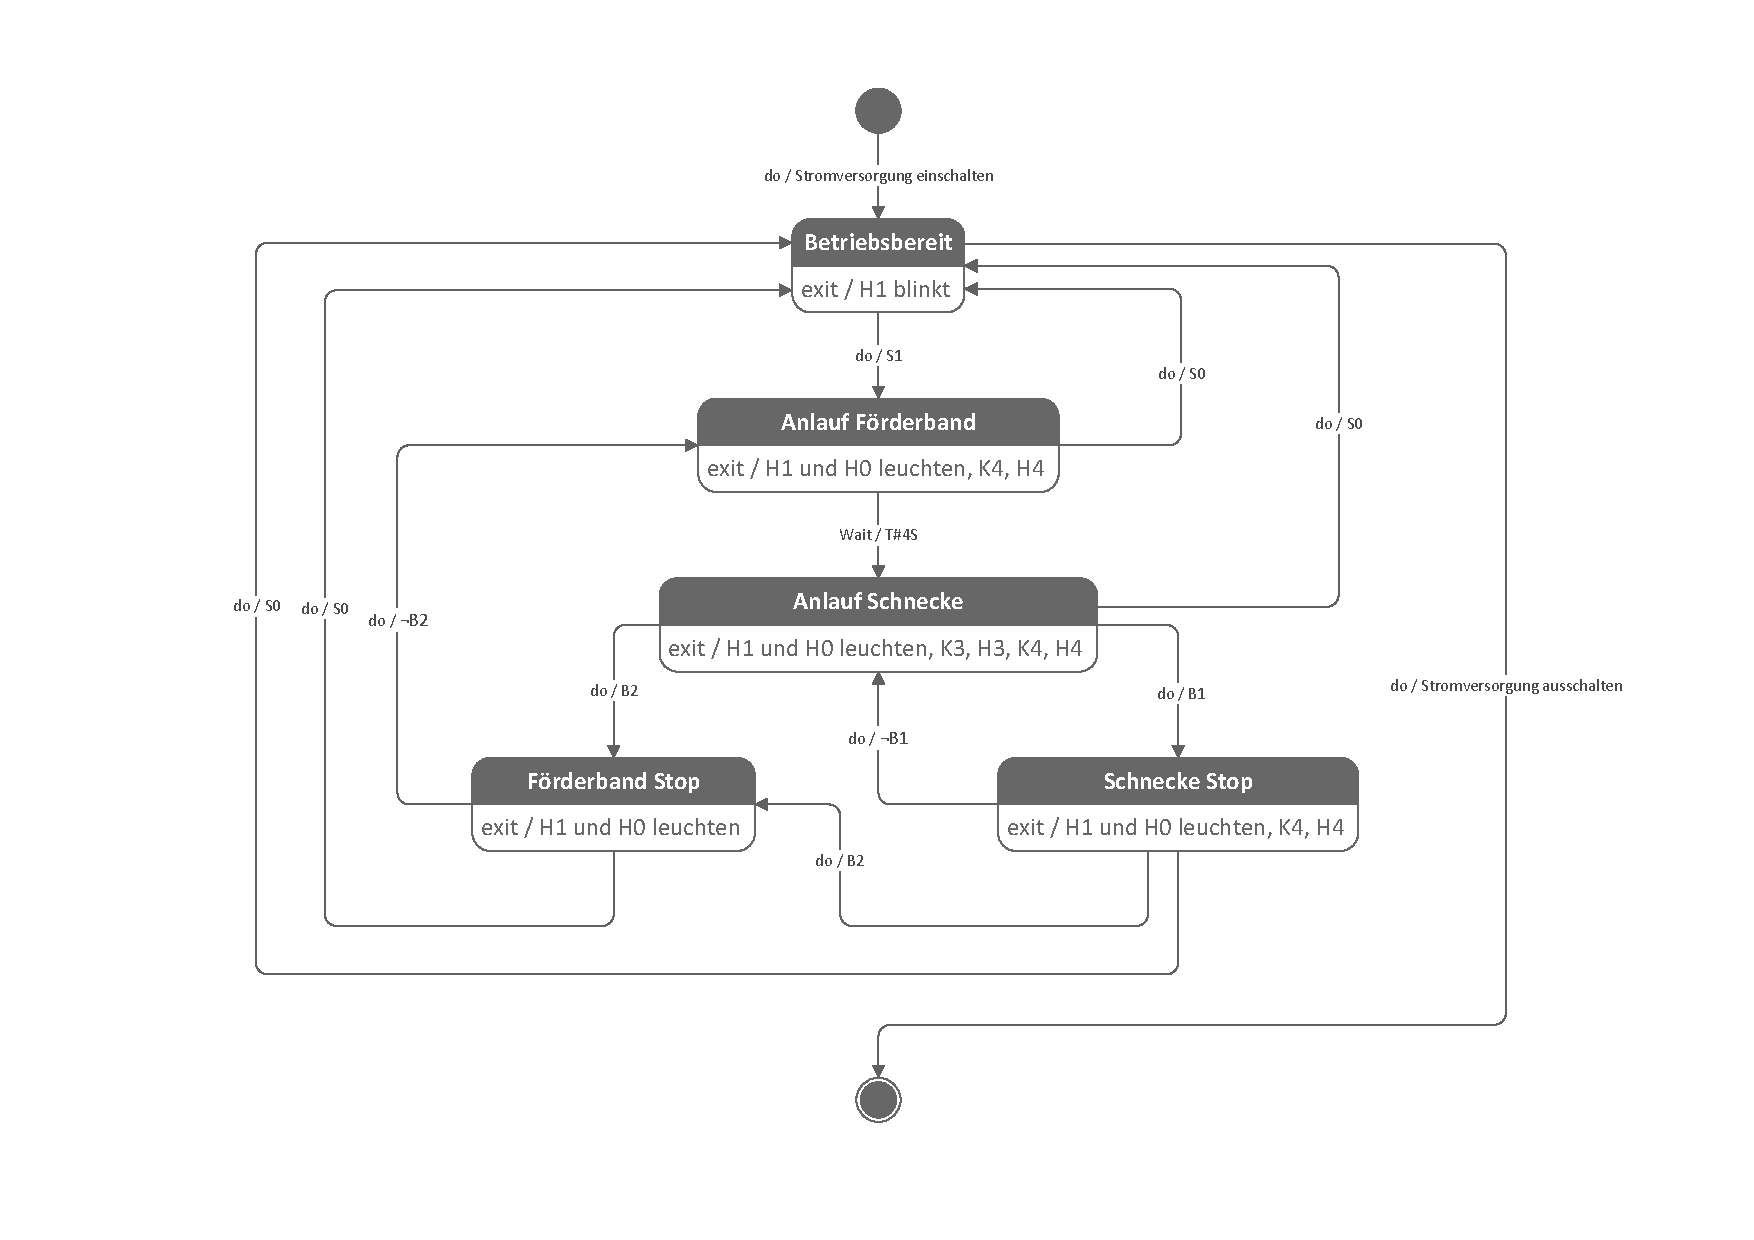
\includegraphics[width=1.0\textwidth]{Bilder/Normalbetrieb.pdf}
   \caption[Automatengraph Normalbetrieb]{Moore Automatengraph des Normalbetriebs (Platzhalter)}
   \label{fig:Bild2}
\end{figure}

\begin{figure}[H]
   \centering
   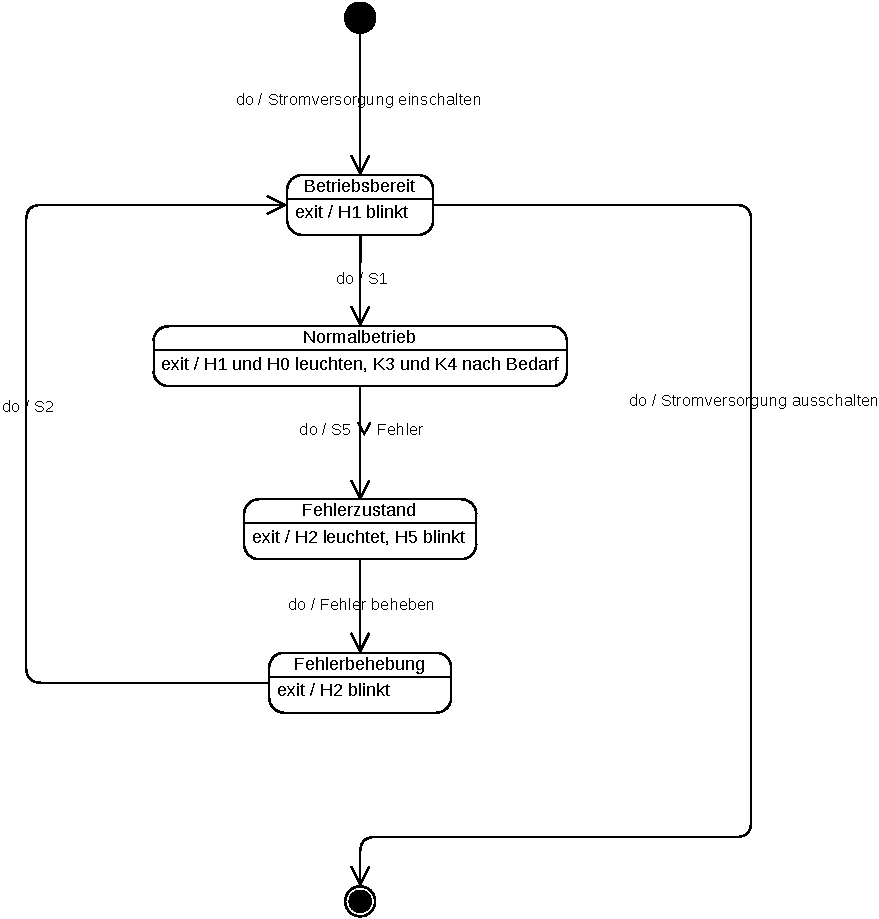
\includegraphics[width=0.8\textwidth]{Bilder/Fehlerfall.pdf}
   \caption[Automatengraph Fehlerfall]{Moore Automatengraph des Fehlerfalls (Platzhalter)}
   \label{fig:Bild3}
\end{figure}

%---------Quellen---------------------------------
\newpage
\newcount\Quellennummer
\Quellennummer=1

\renewcommand\refname{Literaturverzeichnis}
\addcontentsline{toc}{section}{Literaturverzeichnis}

\begin{thebibliography}{999}
{\setlength{\emergencystretch}{3cm}%

\bibitem[\the\Quellennummer]{HTWgross}
HTW-Logo auf dem Deckblatt\par
\url{https://de.wikipedia.org/wiki/Datei:Logo_HTW_Berlin.svg} \par
 Stand: 17.08.2018 um 14:49 Uhr

\advance\Quellennummer by 1
 
\bibitem[\the\Quellennummer]{HTWklein}
HTW-Logo in der Kopfzeile\par
\url{http://tonkollektiv-htw.de/} \par
 Stand: 17.08.2018 um 14:53 Uhr

\advance\Quellennummer by 1

}
\end{thebibliography}

\end{document}
